\documentclass[12pt,a4paper]{report}
%====================== PACKAGES 



%TImes new roman
\usepackage{times} 

\usepackage[french]{babel}
\usepackage[utf8]{inputenc}

% Pour le footer et le header
\usepackage{xcolor}
\usepackage{titlesec}
\usepackage{titleps}


%pour la mise en page des tableaux
\usepackage{tabularx}

\usepackage{ifpdf}
\usepackage{ae}

%police et mise en page (marges) du document
\usepackage[T1]{fontenc}

\usepackage[final]{pdfpages}
\usepackage{tikz}
\usepackage{verbatim}
\usetikzlibrary{arrows,shapes}
\usepackage{algorithm}
\usepackage{algorithmic}
\usepackage{vector}
\usepackage{color}
\usepackage{subfigure}
\usepackage{lettrine}
\usepackage{geometry}
%%%%%%%%%%%%%%%%%%%%%%%%%


%===============Mes couleurs
\definecolor{MyBleue}{RGB}{0, 191, 255}

\textheight=675pt
\textwidth=450pt
\marginparwidth=1pt
\topmargin=.5pt
\oddsidemargin=3pt
\marginparsep=1pt

%%%%%%%%%%%%%%%%%%%

\usepackage{lipsum}
%%%%%%%%%%%%%
\usepackage[hypcap]{caption}

%pour les informations sur un document compilé en PDF et les liens externes / internes
\usepackage{hyperref}
%%%%%%%%%%%%%%%%%%%%%%%%%%%%%%%%%%%%%%%%%


\usepackage{fancyhdr}


%%%%%%%%%%%%%%%%%%%%%%%%%%
\renewcommand{\baselinestretch}{1.5}


\graphicspath{{images/}}


%=========cadre des noms des chapitres et
\usepackage[Glenn]{fncychap}


%==================== DEBUT DU DOCUMENT ===============
\begin{document}

%régler l'espacement entre les lignes


%====================page de garde===================
\thispagestyle{empty}
\newgeometry{top=0.5cm,bottom=1.5cm}
\begin{titlepage}
\begin{center}

% Upper part of the page. The '~' is needed because only works if a paragraph has started.

\includegraphics[width=1\textwidth]{ministere}~\\[1cm]


\includegraphics[width=0.60\textwidth]{isi}~\\[1cm]


\includegraphics[width=0.60\textwidth]{ISI_abreviation}~\\[.5cm]

{\huge \bfseries  STAGE D'\'{E}T\'{E}}\\[1cm]

\begin{LARGE}
{\textbf{R\'{e}alis\'{e} par : }}\\
\end{LARGE}
 


\begin{large}
Yahya HARRATHI \\[.5cm]
\end{large}
% Title
{\color{MyBleue}\hrule }~\\


{\huge \bfseries R\'{e}alisation d'une application web pour la gestion des Allocations pour Voyage d'Affaire  \\[0.4cm] }

{\color{MyBleue}\hrule}~\\

\textbf{Organisme d'accueil :}\\

Soci\'{e}t\'{e} le Monde Informatique


\textbf{encadrant \'{a} l'entreprise : } 
M. Mohamed Anis ZEMNI

\textbf{encadrant \`{a} l'ISI : } 
M. Fahem KEBAIR

\vfill

% Bottom of the page
{\large Ann\'{e}e Universitaire 2015-2016}

\end{center}
\end{titlepage}
\restoregeometry

%page blanche
\newpage
~
%ne pas numéroter cette page
\thispagestyle{empty}
%===============Dédicasse================

\newpage

include Dédicace
%ne pas numéroter cette page
\thispagestyle{empty}

%================Remerciments================
\newpage
\fancyhf{}% Clear header/footer

remerciment

\thispagestyle{empty}
%================Tables des matières==============

\newpage
%ne pas numéroter le sommaire

\tableofcontents

\thispagestyle{empty}

%=================Listes des figures==============

\newpage
%ne pas numéroter le sommaire

\listoffigures
\thispagestyle{empty}
%===============Listes des tableaux============
\newpage
%ne pas numéroter cette page
\listoftables
\thispagestyle{empty}





%====================== INCLUSION DES PARTIES ========
\newpage
~
%recommencer la numérotation des pages �  "1"
\setcounter{page}{0}
\thispagestyle{empty}

\newpage



\chapter{Spécification des besoins}

\setcounter{page}{1}
\thispagestyle{empty}

\newpage

%================header and footer============

\fancyhf{}% Clear header/footer
\newpagestyle{ruled}
{\sethead{}{}{Spécifications des besoins}\headrule
  \setfoot{ISI : Institut Supérieur d'Informatique}{}
  { \thepage}\footrule}
\pagestyle{ruled}

\renewcommand\makeheadrule{\color{cyan}\rule[-.3\baselineskip]{\linewidth}{2.5pt}}
\renewcommand\makefootrule{\color{cyan}\rule[\baselineskip]{\linewidth}{2.5pt}}


%==============Début

 \section{Description du projet}
Le projet consiste à développer une application web pour la gestion des Allocations pour Voyages d'Affaires (AVA) destinée aux clients de la banque STB.
L'AVA permet aux clients de disposer d'une enveloppe de devises transférables destinée à couvrir les frais de leurs voyages / séjours à l'étranger dans le cadre de leurs activités professionnelles.
L'application doit être sécurisée au niveau des échanges des messages et au niveau accès au contenu.
 
 \section{Identification des besoins fonctionnels}

Les besoins fonctionnels doivent répondre aux points précis du cahier des charges qui présente les exigences du futur outil en termes de fonctionnalités. Ce sont une sorte de contrat ou de promesse entre l'utilisateur et le développeur. Les fonctionnalités qui doivent être fournit par mon application sont les suivantes : 

\begin{itemize}
\item \textbf{L'accès et l'identification.}

\begin{itemize}
\item  L'application traite l'accès des utilisateurs.
\item Chaque utilisateur a une interface unique.
\end{itemize}



\item \textbf{Demande d'ouverture d'un dossier AVA.}

%========2eme liste integrée
\begin{itemize}
\item \textbf{Les types d'Allocation :}
L'Allocation pour Voyages d'Affaires peut prendre plusieurs formes :

%======3eme niveau
\begin{itemize}
\item A.V.A exportateur : 
Le montant de l'allocation est fixé actuellement à 25\% des recettes d'exportation de biens ou de services (Vente directe ou indirecte)
sans dépasser un plafond annuel de Cinq Cents Mille (500.000,000) dinars.

\item A.V.A importateur :
Le montant de l'allocation est déterminé à partir du montant des importations réalisées durant l'année précédente.\\
L'allocation est comprise entre 5000 et 50000 dinars.

\item A.V.A autres activités :

Le montant de l'allocation est déterminé à partir du montant du Chiffre d'affaires hors taxes déclaré de l'année précédente.\\
L'allocation est comprise entre 3000 et 30000 dinars.

\item A.V.A nouveau promoteur :
Le montant de l'allocation est fixé à Quinze Mille (15.000) dinars.\\
L'allocation est accordée une seule fois pour toute la période relative à la réalisation du projet.\\
Une fois le quota épuisé, le dossier est clôturé et le client peut choisir une autre catégorie d'AVA

\item A.V.A marchés réalisables à l'étranger :
Le montant de l'allocation est fixé à 15\% du prix du contrat de marché à titre duquel l'allocation est demandée .

\end{itemize} %3eme niveau
\end{itemize} %2eme niveau


Le client peut  demander d'ouvrir un dossier AVA (Exportateur, Importateur, Autres Activités, Nouveau Promoteur, Marché réalisable à l'étranger) en remplissant un formulaire .

%=============Revenir au premiere liste==================
\item \textbf{Consulter l'avancement des dossiers AVA.}
Un dossier AVA a plusieurs états :
\item \textbf{Annulation de voyage.} 
Le client a le droit d'annuler sa voyage et de retourner l'argent dans le dossier AVA, dans un délai de 30 jours. 

\item \textbf{Rétrocession.} 
Après le retour du client d'une voyage d'affaire, il peut faire une rétrocession de l'argent restantes,dans un délai de 7 jours de son retour.
\item \textbf{Gérer les Bénéficiaires.}
Les sociétés clientes du STB peuvent gérer ses employés en changeant leurs etats à : désactivé,à activer, actif ou non actif.

\item \textbf{Demander frais de voyage.}
Les Bénéficiaires d'allocations peuvent demander les frais de voyage en ligne.


\end{itemize}
 
 \section{Identification des besoins non fonctionnels} 
 Outre que les besoins fonctionnels, il faut tenir compte des certains besoins non fonctionnels nécessaires pour une exploitation simple et consistantes des différentes fonctionnalités offertes :
 
 \begin{itemize}
 \item La rapidité de traitement : optimisation de temps de réponse s'approche le plus possible de temps réel.
 
 \item La convivialité : l'application doit être facile à utiliser. En effet, l'interface utilisateur doit être conviviale c'est-à-dire simple, ergonomique et facile à utiliser.
 
 \item L'ergonomie des interfaces hommes -machine (IHM) : l'ergonomie est définie comme l'ensemble des connaissances pour concevoir des applications qui puissent être utilisée avec le maximum d'efficacité et de sécurité. Notre application doit être d'une part utile (répond aux besoins utilisateurs) et d'une autre part utilisable (facile à utiliser).
 Pour ce fait, nous devons respecter les critères de qualité des interfaces.

\item Le système doit être une solution informatique performante dans la bonne circulation de l'information et du travail.
 
 \end{itemize}
 \section{Diagramme des cas d'utilisations global}
 
 \begin{figure}[!h]
\begin{center}

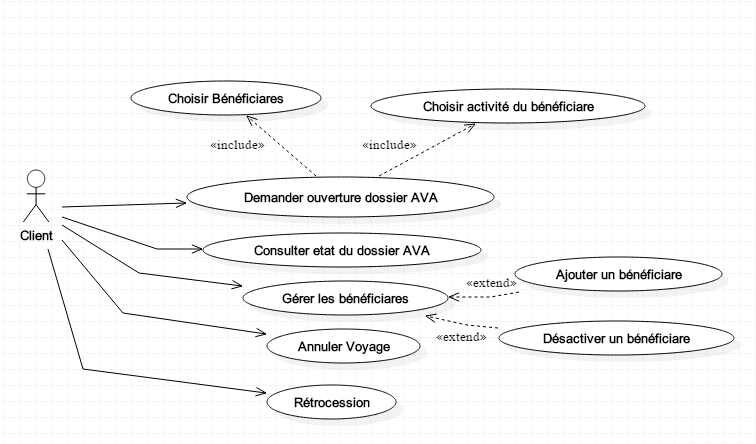
\includegraphics[width=10cm]{./conception/Global_use_case}

\caption{Diagramme des cas d'utilisations global}
\end{center}
\end{figure}

 
 \section{Identifications des acteurs et des cas d'utilisations}
 
 
 
 \begin{table}[!h]
\begin{center}
\begin{tabular}{|l|l|}
\hline 
Acteur & Type \\ 
\hline 
Client & Principale \\ 
\hline 
Bénéficiaire & Principale \\ 
\hline 
STB & Principale \\ 
\hline 
\end{tabular} 
\end{center}
\caption{Tableau d'identification des acteurs.}
\end{table}


 
%new table


\begin{comment}
\begin{table}[!h] 
\begin{center}
\begin{tabular}{ |c|c| } 
\hline
Acteur &  Cas d'utilisation  \\
\hline
\multirow{5}{*}{Client} & Ouverture dossier AVA  \\ 
& Consulter état dossier AVA  \\ 
& Gérer bénéficiaires  \\ 
& Annuler un voyage \\
& Rétrocéder \\


\hline STB & Principale \\ 
\end{tabular}
\end{center} 
 \caption{Tableau d'identification des acteurs.}
\end{table}
 \end{comment}

%chap2
\chapter{Analyse et conception}


\thispagestyle{empty}

\newpage

%================header and footer============


\sethead{}{}{Analyse des besoins}\headrule



%==============Début

 \section{Analyse}
 
\subsection{Modèle du cycle de vie}

\subsection{Raffinement des cas d'utilisations}

   
   \begin{enumerate}[label=(\alph*)]
   \item {Diagramme détaillé de cas d'utilisation \textless  Demander l'ouverture d'un dossier AVA \textgreater}
   
    \begin{figure}[!h]
\begin{center}

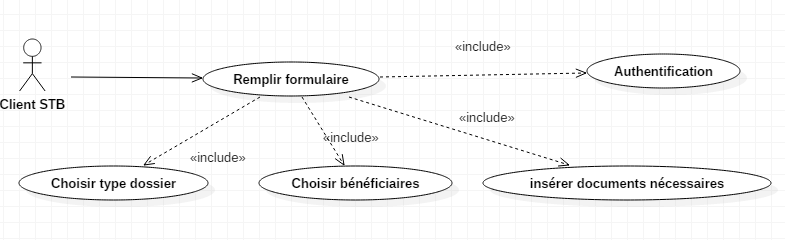
\includegraphics[width=10cm]{./conception/use_case_ouverture}

\caption{Diagramme détaillé de cas d'utilisation demande d'ouverture d'un dossier AVA.}
\end{center}
\end{figure}
 
  Le client du STB peut demander, en ligne, la création d'un dossier AVA en remplissant un formulaire.
Ce dernier contient des informations concernant son type d'activité, compte dans la banque STB, etc.
Le Client peut ajouter des bénéficiaires et choisir leurs états (désactivé, à activer, actif, non actif).
À la fin du formulaire, il doit insérer des fichiers PDF qui varient selon le type du dossier choisi.
 

   
    \item{Diagramme détaillé de cas d'utilisation \textless Annulation de voyage \textgreater}
    
     \item{Diagramme détaillé de cas d'utilisation \textless Rétrocession \textgreater}
     
     \item{Diagramme détaillé de cas d'utilisation \textless Ajouter un Bénéficiaire \textgreater}
     
      \item{Diagramme détaillé de cas d'utilisation \textless Désactiver un Bénéficiaire \textgreater}
    \end{enumerate}    
 


 \section{Conception}
 
 \subsection{Diagrammes d'activités}
 
 \subsubsection{Diagrammes de séquence \textless Demande d'ouverture d'un dossier AVA \textgreater}

\begin{figure}[!h]
 \begin{center}
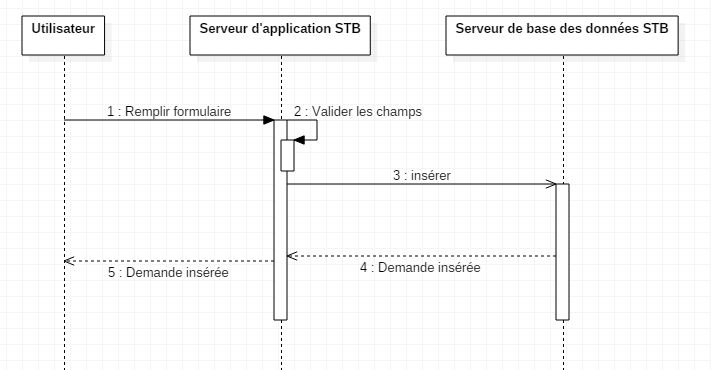
\includegraphics{./conception/sequence_ouverture}

%légende de l'image
\caption{Diagramme de séquence\textless ouverture dossier AVA\textgreater}
\end{center}
\end{figure}

%description textuelle
\begin{itemize}
\item  Description textuelle \\
Titre : Demande d'ouverture d'un dossier AVA.\\
Acteur principal : client du STB.\\
Résumé : Le client du STB doit pouvoir demander en ligne la création d'un dossier AVA.\\

Scénario nominal\\
\begin{enumerate}
\item Le client choisit l'interface d'ouverture d'un dossier AVA.
\item Il remplit un formulaire d'ouverture.
\item Il valide le formulaire.
\item Le système valide les champs saisis.
\item Le système trouve que le client n'a pas un dossier AVA ouvert.
\item Notification de la création de la demande.
\end{enumerate}
\end{itemize}

  \subsubsection{Diagrammes d'activité \textless Rétrocession \textgreater}
  
  \subsection{Diagrammes de séquences}
  
  \subsubsection{Diagramme de séquence \textless s'authentifier \textgreater}
  
  \subsubsection{Diagramme de séquence \textless Ajouter bénéficiaire \textgreater}
  
  \subsection{Diagramme des classes global}
  
  %inclusion d'une mage dans le document
\begin{figure}[!h]


%remplacer "width" par "height" pour régler la hauteur

\begin{center}
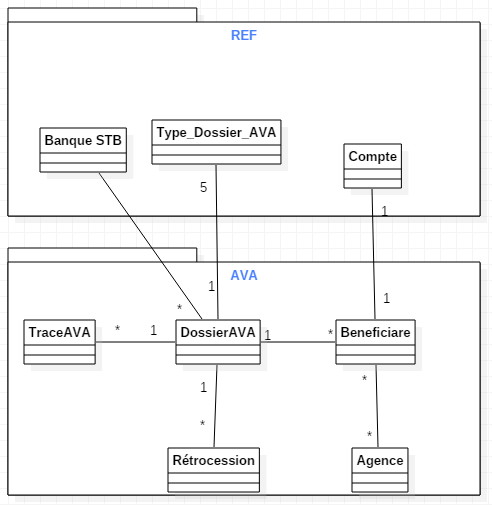
\includegraphics{./conception/diagramme_classes}

%légende de l'image
\caption{Diagramme des classes global}
\end{center}
\end{figure}
  
  
  
  
 

 
 
 

 

\chapter{Réalisation et tests}

\setcounter{page}{1}
\thispagestyle{empty}

\newpage

%================header and footer============

\fancyhf{}% Clear header/footer
\newpagestyle{ruled}
{\sethead{}{}{Réalisation et tests}\headrule
  \setfoot{ISI : Institut Supéerieur d'Informatique}{}
  { \thepage}\footrule}
\pagestyle{ruled}

\renewcommand\makeheadrule{\color{cyan}\rule[-.3\baselineskip]{\linewidth}{2.5pt}}
\renewcommand\makefootrule{\color{cyan}\rule[\baselineskip]{\linewidth}{2.5pt}}

\setcounter{page}{1}
%==============Début
\begin{Large}
Introduction 
\end{Large}

Après avoir élaboré la conception de mon application, j’aborde dans ce chapitre le dernier volet de ce rapport, qui a pour objectif d'exposer la phase de réalisation.\\
Je mène tout d’abord une étude technique où je décris les ressources logicielles utilisées dans le développement du projet.\\
 Je présente en premier lieu mon choix de l’environnement de travail, où je spécifie l’environnement matériel et logiciel que j’ai utilisé pour réaliser l’application puis je détaille l’architecture.\\
Par la suite, je présente quelques interfaces réalisées pour illustrer le fonctionnement de quelques activités du système. 

%\renewcommand{\thesection}{\arabic{section}}
\section{Etude technique}

\subsection{Environnement matériel}
A fin de réaliser le projet, j’ai travaillé sur un ordinateur portable qui a les caractéristiques suivantes :\\ 

\begin{table}[!h]
\begin{center}
\begin{tabular}{|l|l|}
\hline 
Marque & DELL INSPIRON N5040 \\ 
\hline 
Processeur & Intel core i3 @2.20GHZ \\ 
\hline 
Mémoire & 6,00 Go \\ 
\hline 
Système d'exploitation & Windows 8.1 64 bits \\ 
\hline 
\end{tabular} 
\end{center}
\caption{Tableau de l'environnement matériel}
\end{table}

\subsection{Environnement logiciel}
\subsubsection{Outils de développement}
%=================NetBeans================
\begin{itemize}
\item NetBeans JEE\\

%inclusion d'une mage dans le document
\begin{figure}[!h]
\begin{center}
%taille de l'image en largeur
%remplacer "width" par "height" pour régler la hauteur

\includegraphics[width=3cm]{./NetBeans}

%légende de l'image
\caption{Logo NetBeans}
\end{center}
\end{figure}

NetBeans est un environnement de développement intégré(EDI)open source,crié par Sun Microsystems en 2000 \cite{cite1}.

%=================Postman===================
\item Postman


\begin{figure}[!h]
\begin{center}


\includegraphics[width=3cm]{./Postman}

\caption{Logo Postman}
\end{center}
\end{figure}


%=================SQLDevveloper===================
\item SQL Developer


\begin{figure}[!h]
\begin{center}


\includegraphics[width=3cm]{./SQLDeveloper}

\caption{Logo Oracle SQL Developer}
\end{center}
\end{figure}



Oracle SQL Developer est un environnement de développement intégré (EDI) multi-plateforme, fourni gratuitement par Oracle Corporation et utilisant la technologie Java (Java Development Kit). C'est un outil graphique permettant d'interroger des bases de données Oracle à l'aide du langage SQL.

\end{itemize}

%=============================Outils de modélisation

\subsubsection{Outils de modélisation}

\begin{itemize}
\item StarUML


\begin{figure}[!h]
\begin{center}


\includegraphics[width=3cm]{./StarUML}

\caption{Logo StarUML}
\end{center}
\end{figure}


StarUML est un logiciel de modélisation UML, écrit en Delphi. il est facile à utiliser, propose plusieurs générateurs de code et gère la plupart des diagrammes spécifiés dans la norme UML 2.0.\cite{cite2}

\end{itemize}






\newpage

\bibliographystyle{alphadin}
\bibliography{bibliographie}


\end{document}
